

\section{Global Training Dynamics}
% The invariants $\delta_i$ allow us to present a concrete framework for understanding the global dynamics of neurons in terms of their initialization. We can understand the global dynamics of neural networks in terms of two regimes corresponding to eigenvectors of $M_\delta$ in the previous section: \emph{Radial training} and \emph{Tangential training}. 

In this section, we consider the extreme cases of initialization: $\delta \ll -\|\xi\|$ (radial dynamics) and $\delta \gg \|\xi\|$ (tangential dynamics). This corresponds to training only the bottom and only the top layer of the network, respectively. 

% We show that lazy training occurs when $\delta \ll 0$ (radial motion in the reduced parameters). We demonstrate that in this regime, the network is biased towards ``smooth'' solutions. At the other end of the spectrum \cite{maennel2018gradient} observe that small initializations lead to a quantization effect of the weight vectors independent of the size of the network. This phenomenon occurs more prominently as $\delta$ grows larger. Furthermore, we describe precisely where the the weight vectors concentrate in terms of the input samples. We also note that the samples at which neurons concentrate are not fixed, but are dynamical quantities which depend on the activation pattern and on the residuals.

% We note that scaling the gradient flow is equivalent to scaling the distributions from which the initial parameters, $\theta$ are sampled, thus we can control the value of $\delta$ by either rescaling the gradient flow or changing the initial distribution of $\theta$.


\subsection{Radial Training}

\note{We should say that radial training is what happens with the standard initialization using pytorch}

In pure radial regime, we are only learning the outer layer parameters and leaving the inner parameters fixed. This corresponds to \emph{kernel learning}~\note{Cite someone}. In the overparameterized setting, we wish to solve

\begin{equation}\label{eq:lsq_overparameterized}
\begin{gathered} 
    \text{minimize } ||c||^2\\
    \text{subject to } M_x(a, b) c = y
\end{gathered}
\end{equation}

which is strictly convex with convex constraints. Writing $M = M_x(a,b)$, we have that solution to \eqref{eq:lsq_overparameterized} is given by $c = M^T (M M^T)^{-1} y$. We define the kernel

\begin{equation}
    K_{(a,b)}(x,x') = \sum_{i=1}^m [a_i x + b_i]_+[a_i x' + b_i]_+
\end{equation}


The optimized function is given by

\begin{equation}
    f(x) = \sum_{j=1}^s v_j K(x_j, x)
\end{equation}


where $v = K(x_i,x_j)^{-1} y$. Of course, this closed form solution only corresponds to the point of convergence of the gradient flow only if $c(0) = 0$. The more general dynamics of the flow can be similarly derived in terms of the kernel $K$ (see Appendix). Furthermore, it is known in this setting that early stopping for
gradient descent will act as a regularizes as these eigenfunctions of $K$ typically correspond to lower frequency features of the function being fit \note{cite}.







\paragraph{Infinite width limit}
% We analyze the behavior of the \emph{limit kernel} as the number of weights $m \rightarrow \infty$ in the radial regime. We show that the overparameterized least squares problem in this setting minimizes curvature. Furthermore, for 1D functions, the network functions are natural cubic spines. 
In the infinite width ($m = \infty)$ limit, the parameters, $\theta$ become densities $\theta(s) = (a(s), b(s), c(s))$. Assuming that $s \in [k_1, k_2], x \in [k_1, k_2]$, then we can write the function $f$ as

\begin{equation}
    f(x) = \int_{k_1}^{k_2} c(s) [a(s) x + b(s)]_+ ds
\end{equation}

and the least squares problem becomes
\begin{equation}
    \begin{gathered}
    \text{minimize } ||c(s)||^2\\
    \text{subject to } \int_{k_1}^{k_2} c(s) [a(s)x_i + b(s)]_+ ds = y_i
    \end{gathered}
\end{equation}

\begin{lemma}\label{le:curvature}
The second derivative of $f(x)$ is the parameter density $c(s)$. i.e. 
\begin{equation*}\partial_x^2 f(x) = c(s)\end{equation*}
\end{lemma}
\begin{proof}
\todo{TODO}
\end{proof}

Thus, the quantity $||c(s)||^2 = ||\partial_x^2 f(x)||^2$ being minimized is the \emph{curvature}. Thus, we can view the radial regime as an implicit bias towards ``smooth'' functions.



For 1D functions with knots initialized from a uniform distribution, we give an exact equation for the limit kernel. 

\begin{lemma}\label{le:cubic_spline}
Assume that the knots $e(s) =\ -\frac{b(s)}{a(s)} ~ U(k_1, k_2)$, then the inifinite width kernel, $K(x, y)$ is a cubic polynomial in $x$ and $y$
\end{lemma}
\begin{proof}

We can rewrite the kernel,
\begin{equation}
    K(x, y) = \int_{k_1}^{k_2} [a(s)x + b(s)]_+ [a(s)y + b(s)]_+ ds
\end{equation}

in terms of the knots $e(s)$

\begin{equation}
    K(x, y) = \int_{k_1}^{k_2} \tau(x, s) \tau(y, s) a(s)^2 (x - e(s)) (y - e(s)) ds
\end{equation}

where $\tau(x, s) = \mathds{1}[a(s)x + b(s) \geq 0]$. $a(s)$. Sicne the knots $e(s) = -\frac{b(s)}{a(s)}$ are uniformly distributed, we can write $e(s) = s$ which implies $-b(s) = s a(s)$. In this case, we can assume without loss of generality that $v(s) = -s$ and $u(s) = 1$. We then rewrite the kernel

\begin{equation}
    \begin{aligned}
    K(x, y) &= \int_{k_1}^{k_2} \tau(x, s) \tau(y, s) (x - s) (y - s) ds\\
            &= \int_{k_1}^{\min(x, y)} (x - s) (y - s) ds\\ 
            &= s xy - \frac{1}{2} s^2 (x + y) - \frac{1}{3} s^3 \bigg\rvert_{k_1}^{\min(x, y)}
    \end{aligned}
\end{equation}

which is a cubic function in $x$ and $y$.
\end{proof}

Recall that for full rank $M_x(a,b)$, the function $f(x)$ interpolates the samples, $x_i$. Thus, a corollary to Lemmas \ref{le:curvature} and \ref{le:cubic_spline} is that for uniform knot initialization, 1D neural network functions are cubic splines interpolating the samples. Figure~\ref{fig:cubic_splines} shows the convergence to a cubic spline as the number of neurons grows large. \note{We need to cite the paper on linear splines here.} 

\begin{figure}\label{fig:cubic_splines}
    \centering
    \minipage{0.33\textwidth}
    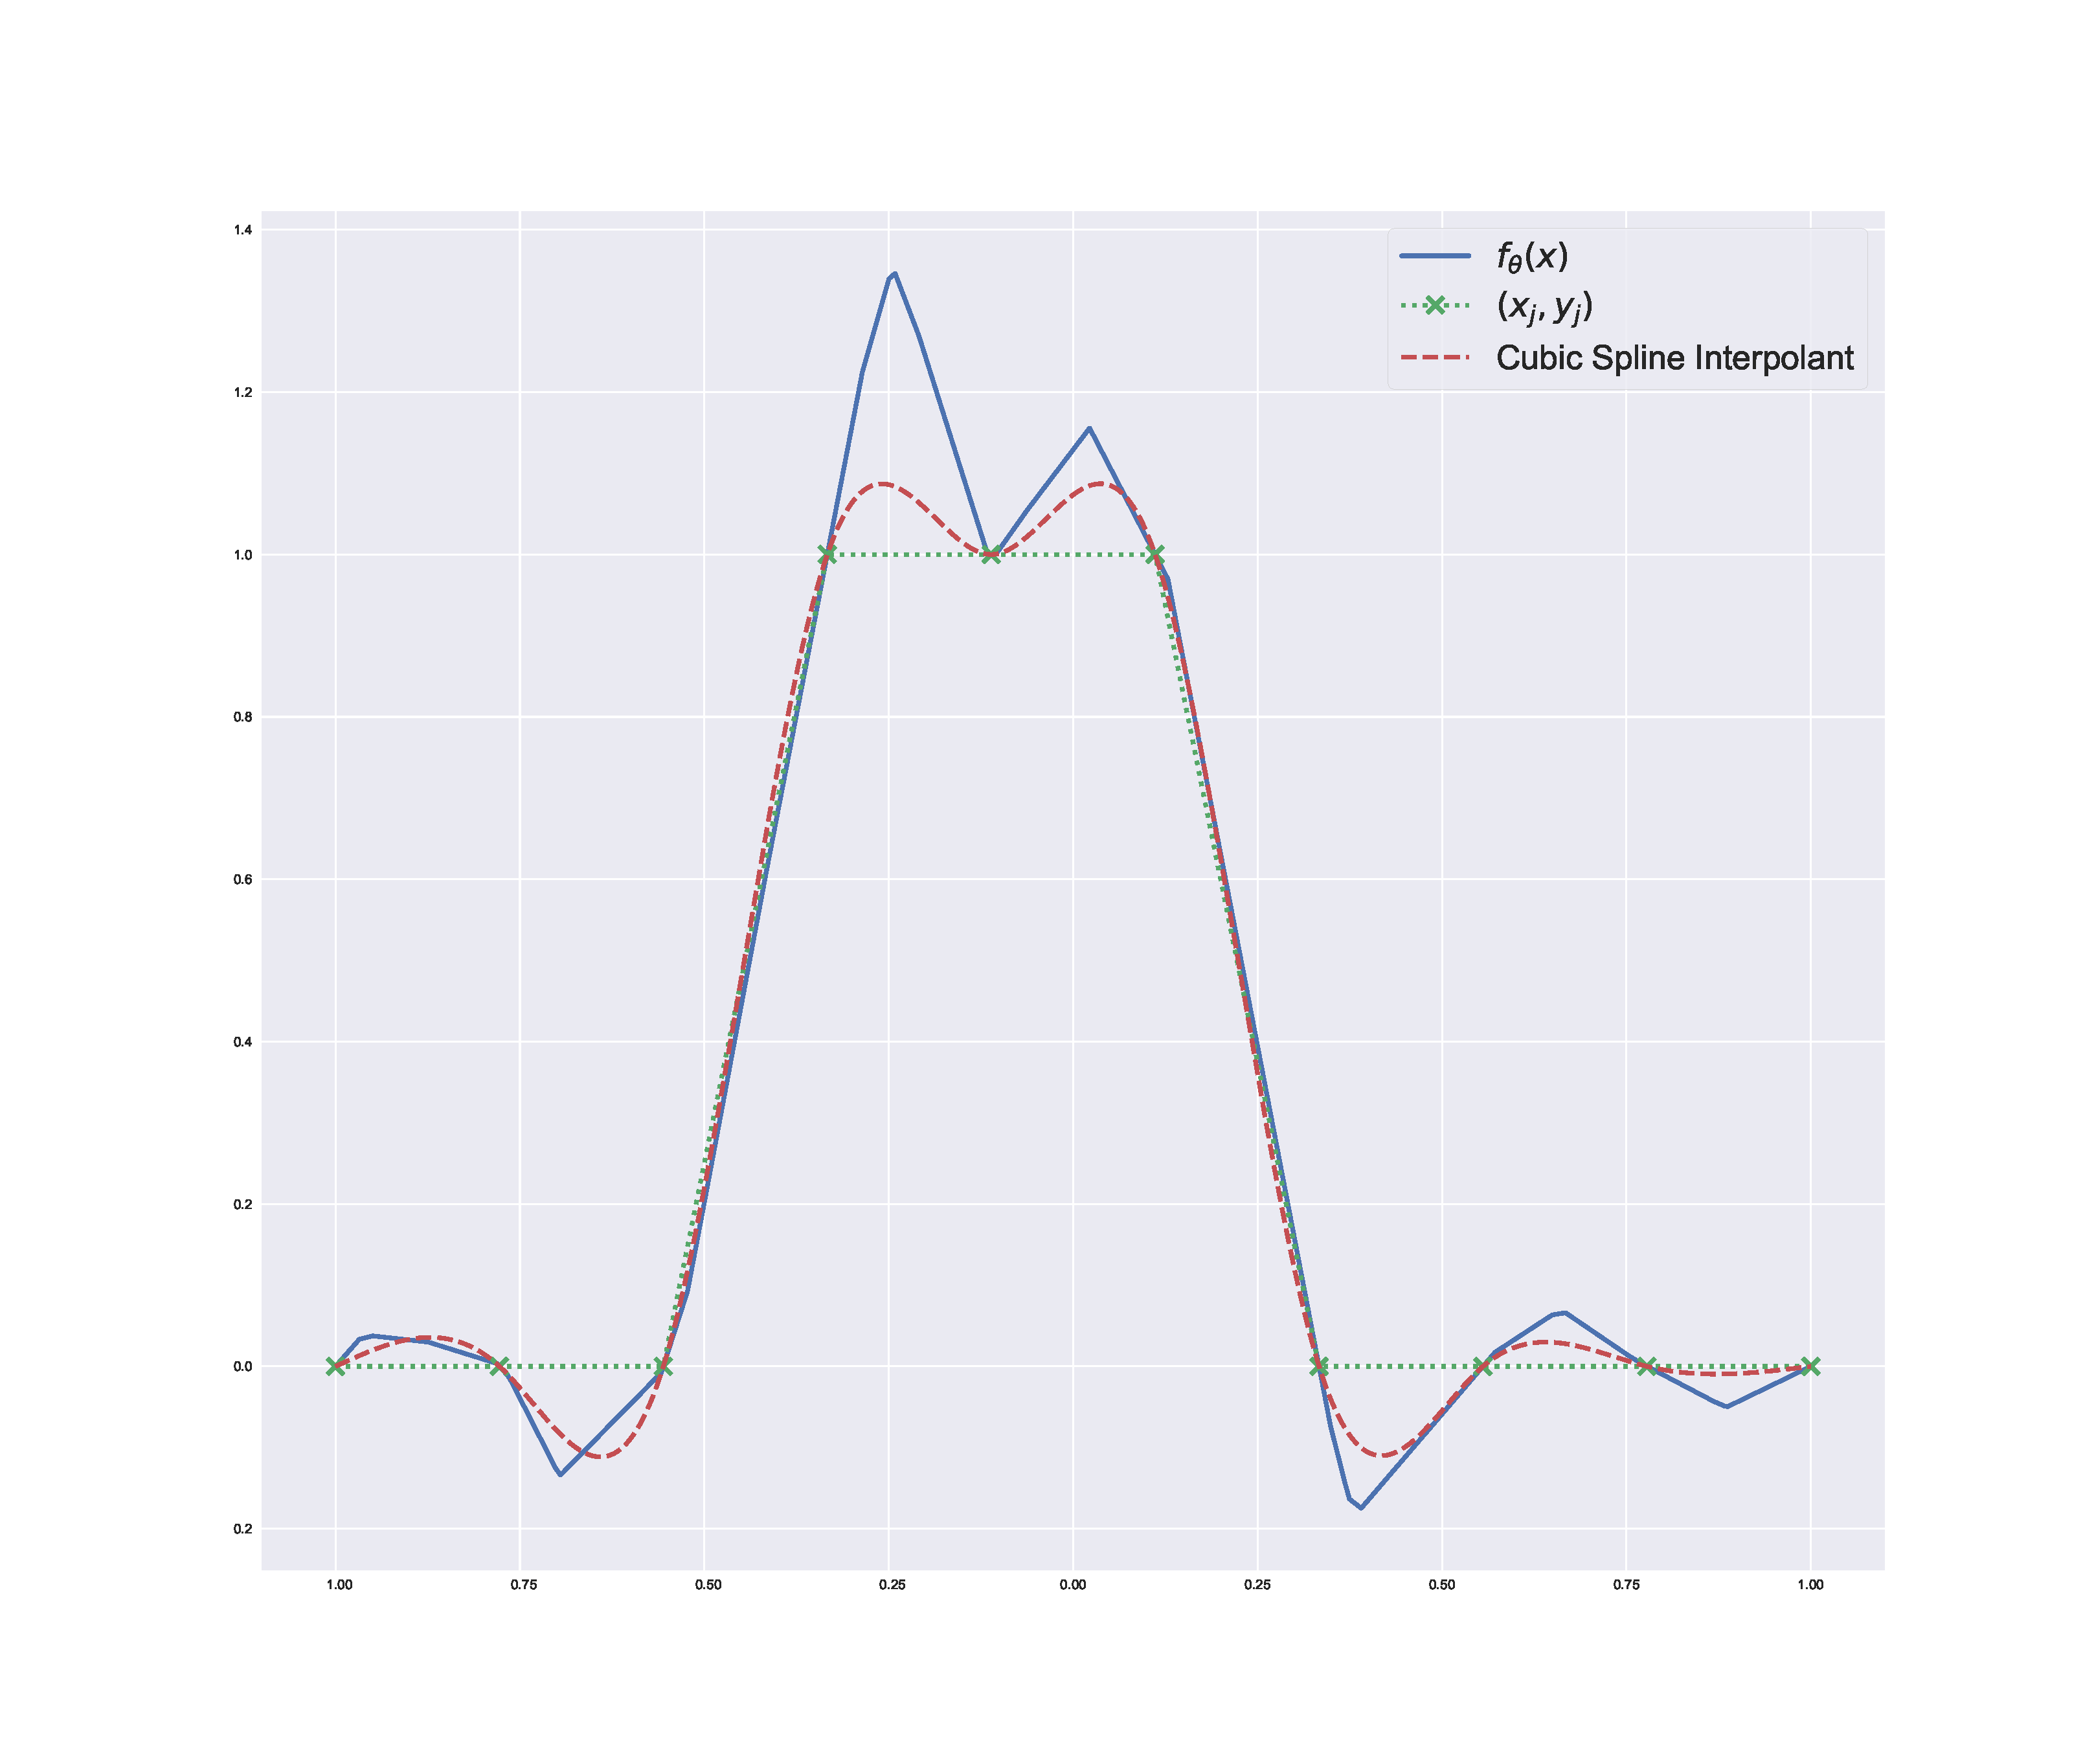
\includegraphics[width=\linewidth]{figures/cubic_spline100.pdf}
    \endminipage\hfill
    \minipage{0.33\textwidth}
    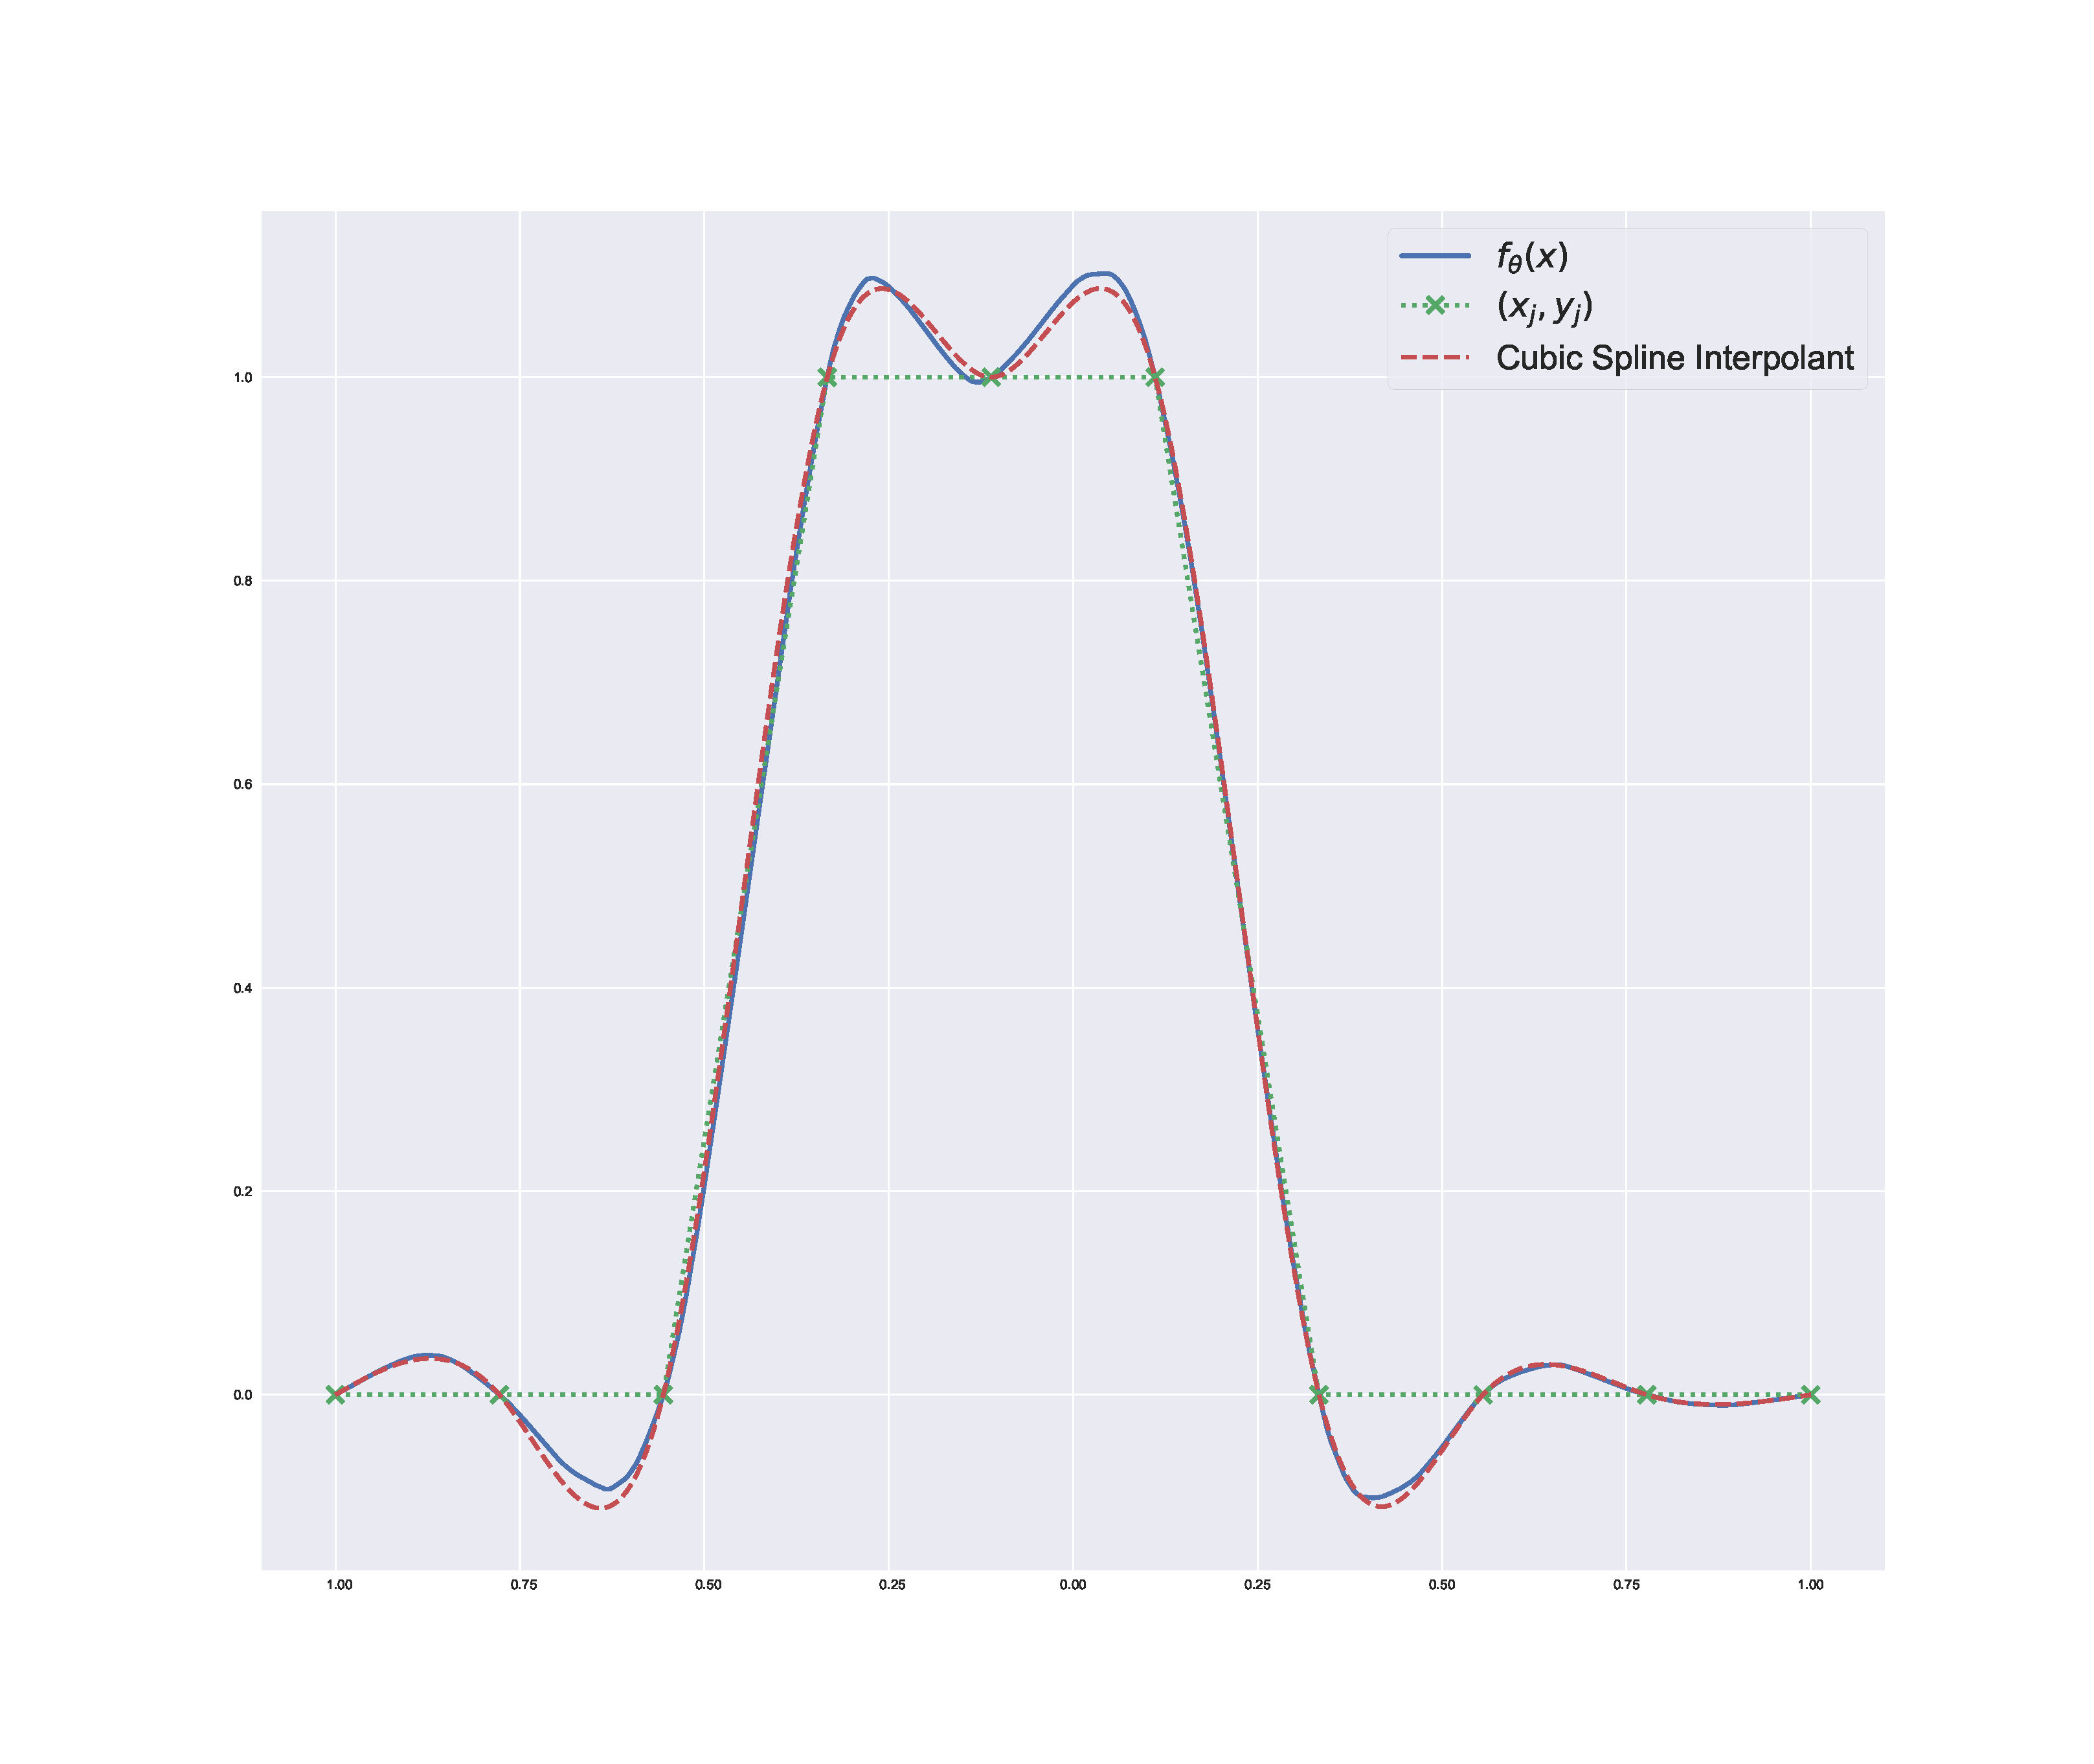
\includegraphics[width=\linewidth]{figures/cubic_spline_1k.pdf}
    \endminipage\hfill
    \minipage{0.33\textwidth}
    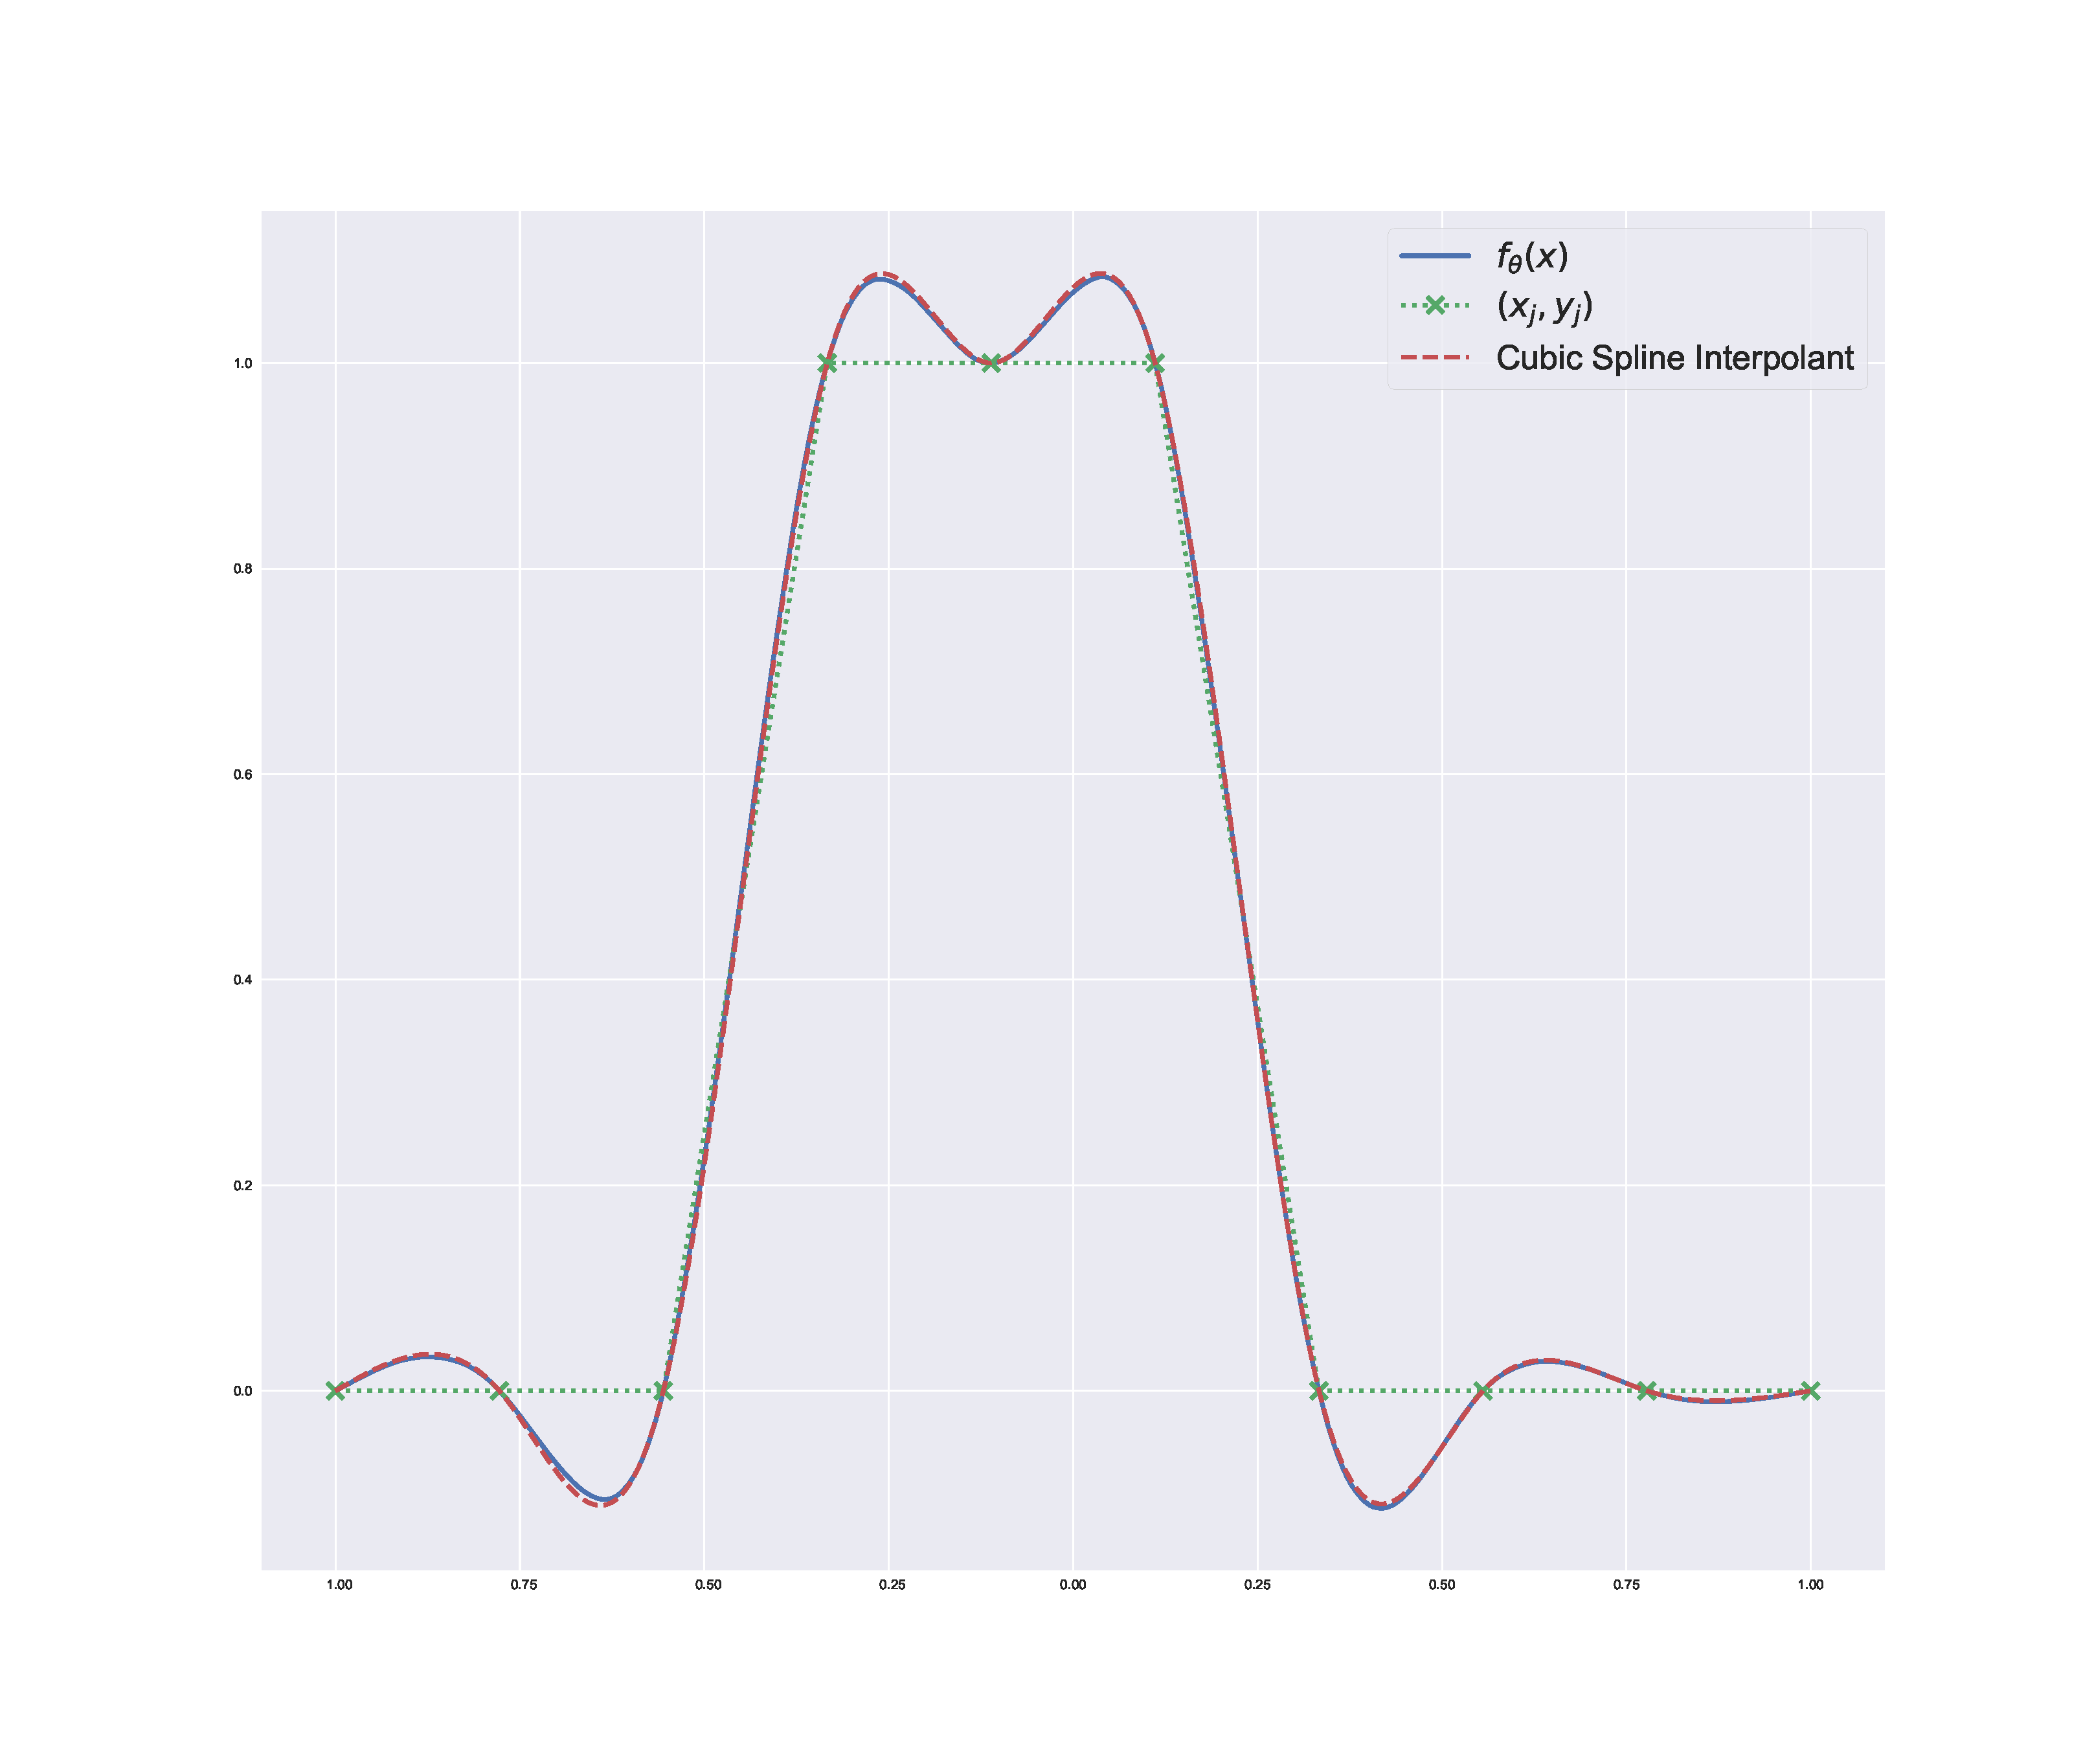
\includegraphics[width=\linewidth]{figures/cubic_spline_10k.pdf}
    \endminipage
    \caption{Regression in the purely tangential regime ($\delta = -\infty$) using varying knots. We observe that as the number of knots increases, the function, $f_\theta$ converges to a cubic spline interpolant with $\partial_x^2 = 0$ on the boundary.}
    \label{fig:radial_trajectores}
\end{figure}



















\subsection{Tangential Training, $\delta \gg \|\xi\|$}


\note{Use interesting?}

Recall that Lemma~\ref{le:pw_continuous} states that the gradient field $\nabla \tilde{L}$ is piecewise continuous. An important consequence of this result is that the gradient field could point in opposite directions on the boundary of a sample (\todo{Figure \ref{fig:todo}}). In this case, a neuron could get stuck along the boundary for that sample and only be able to move radially. We call the samples at which neurons get stuck \emph{attractive}. The existence of attractive samples leads to neurons piling up at samples, biasing the functions $f(x)$ to be piecewise linear with a small number of pieces.

We now give a precise condition for when a sample is attractive. We also show that the set of attractive samples is a dynamical quantity which depends only on the activation.

Recall that in the reduced parameter space, a sample $x_i$ corresponds to a line in the $(u, v)$ plane. The sample $x_i$ is \emph{attractive} if the loss gradient in the reduced parameters $\nabla \tilde{L}$ points in opposite directions on either side of this line. 

Formally, we can express attractiveness as a condition on the time derivative of the knots $e_i(t)$. 

\begin{equation}\label{eq:moving_knots}
\partial_t e_i(t) = \frac{-a_i \partial b_i + b_i \partial a_i}{a_i^2} = c_i\frac{- a_i \sum_
{j=1}^s
\tau_{ij} r_j + b_i \sum_
{j=1}^s \tau_{ij} x_j r_j}{a_i^2} = \frac{\sum_{j=1}^s \tau_{ij}c_i(-a_i
+x_j b_i)r_j}{a_i^2}
\end{equation}

\note{Possibly useful to frame attractiveness/interestingness:}
\begin{definition}
Consider a function of the form $h(\bm w) = \sum_{i=1}^s r_i [\langle \bm w,\bm x_i\rangle ]_+$ with $\bm w, \bm x_i \in \RR^2$ and $r_i \in \RR$. We say that $\hat{ \bm w} \in \mathbb S^1$ is a \emph{stable direction} if $\hat{ \bm w} \in \alpha \partial h(\hat {\bm w})$ for some $\alpha > 0$ (perhaps give more intuitive definition/picture?).
\end{definition}

A stable direction can either be on the boundary or on the internal part of a segment. From~\eqref{eq:moving_knots}, we are interested in the stable directions for $h((a_i,b_i)) = \epsilon_i \sum_{i=1}^s r_j [(-a_i + x_jb_j)]_+$. Stable directions on the boundaries are ``interesting points''.


\note{Think about how to present this}

Assume that the samples $x_1 < x_2 < \ldots < x_s$ are ordered and suppose that the knot $e_i$ lies on the sample $x_k$, i.e. $e_i(t) = x_k$. Denoting $r = (r_j(\theta))_{j=1}^s$ as the vector of residuals, we have that a the sample $x_k$ is attractive if

\begin{equation}
\begin{aligned}
    &\sum_{j=1}^{k-1} (1+x_j x_k) r_j \lessgtr 0 \quad \mbox{ and } \qquad \sum_{j=1}^k (1+x_j x_k) r_j \gtrless 0, \quad \mbox{ or }\\
    &\sum_{j=k}^s (1+x_j x_k) r_j \gtrless 0 \quad \mbox{ and } \qquad \sum_{j=k+1}^{s} (1+x_j x_k) r_j \lessgtr 0.\\
\end{aligned}
\end{equation}

If $z_j = (1,x_j) r_j$, we can rewrite this as

\begin{equation}
\begin{aligned}\label{eq:attractor_cond}
    &\sum_{j=1}^{k-1} \langle z_k , z_j \rangle < 0 \quad \mbox{ and } \qquad \sum_{j=1}^{k} \langle z_k, z_j \rangle > 0, \quad \mbox{ or }\\
    &\sum_{j=k}^{s} \langle z_k , z_j \rangle > 0 \quad \mbox{ and } \qquad \sum_{j=k+1}^{s} \langle z_k, z_j \rangle < 0.\\
\end{aligned}
\end{equation}


This can be written in terms of the Gram matrix $Z_{ij} = (\langle z_i, z_j\rangle)$.

\paragraph{Dynamics of Attractive Samples}

The attractiveness condition \eqref{eq:attractor_cond} is a dynamic quantity depending on the residuals $r(\theta)$ as well as the samples, $x$. A sample can only change from attractive to unattractive or vice-versa when the activation matrix $\tau$ changes.

\begin{lemma}
If the truth value of the condition \eqref{eq:attractor_cond} changes at time $t$, then the activation matrix, $\tau$ must also change at time $t$.
\end{lemma}
\begin{proof}
\todo{TODO}
\end{proof}

Qualitatively, a sample is attractive when there is a large change in sign between the average residual on one side of the sample and the sample itself. Attractive samples on the ''peaks`` and ``valleys of the of the residual. As with the residual case, low frequency features in the data tend to be fit first with high frequency features being fit later. \todo{Figure~\ref{fig:todo}} shows an example of this behavior.



























\iffalse
\subsection{Old}
% It is easy to verify that the eigenvalue-eigenvector pairs of $K(\xi)$ are
% $(\beta a^2+ \beta b^2 + \alpha c^2, (a,b))$ and $(\alpha c^2, (-b,a))$, which correspond to radial and tangential components of $(u, v)$. From this we deduce that


% \begin{itemize}
%     \item If $\alpha c^2 \ll \beta (a^2 + b^2)$, which means that $\delta <
%     0$, then $\xi_i'(t) \propto (a(t),b(t))$, and the reduced neuron
%     moves~\emph{radially}.
%     \item If $\alpha c^2 \gg \beta (a^2 + b^2)$, which means that $\delta > 0$, then
%     $\xi_i'(t) \propto \nabla^\xi(\xi)_i$, so the reduced neuron follows themaybePres
% \end{itemize}



\paragraph{Node dynamics.}

\begin{equation}
\dot e_i(t) = \frac{-\dot b_i a_i + \dot a_i b_i}{a_i^2} = c_i\frac{- a_i \sum_
{j=1}^s
\tau_{ij} r_j + b_i \sum_
{j=1}^s \tau_{ij} x_j r_j}{a_i^2} = \frac{\sum_{j=1}^s \tau_{ij}c_i(-a_i
+x_j b_i)r_j}{a_i^2}
\end{equation}

If $e_i(t) = x_k$, that is, $-b_i = x_k a_i$, then

\begin{equation}
\dot e_i(t) = -\frac{c_i}{a_i}\sum_{j=1}^s \tau_{ij} (1
+ x_j x_k)r_j
\end{equation}

Assuming $x_1 < \ldots < x_s$, we say that a sample point $x_k$ is \emph{attractive} for a residual vector $r$ if

\begin{equation}
\begin{aligned}
    &\sum_{j=1}^{k-1} (1+x_j x_k) r_j \lessgtr 0 \quad \mbox{ and } \qquad \sum_{j=1}^k (1+x_j x_k) r_j \gtrless 0, \quad \mbox{ or }\\
    &\sum_{j=k}^s (1+x_j x_k) r_j \gtrless 0 \quad \mbox{ and } \qquad \sum_{j=k+1}^{s} (1+x_j x_k) r_j \lessgtr 0.\\
\end{aligned}
\end{equation}

If $z_j = (1,x_j) r_j$, we can rewrite this as

\begin{equation}
\begin{aligned}\label{eq:attractor_cond}
    &\sum_{j=1}^{k-1} \langle z_k , z_j \rangle < 0 \quad \mbox{ and } \qquad \sum_{j=1}^{k} \langle z_k, z_j \rangle > 0, \quad \mbox{ or }\\
    &\sum_{j=k}^{s} \langle z_k , z_j \rangle > 0 \quad \mbox{ and } \qquad \sum_{j=k+1}^{s} \langle z_k, z_j \rangle < 0.\\
\end{aligned}
\end{equation}


This can be written in terms of the Gram matrix $Z_{ij} = (\langle z_i, z_j\rangle)$.




\subsection{Denis}
It is best to write $K$ as 
\begin{equation}
c(||\xi||^2)^2 I +  c(||\xi||^2)^{-2}  \xi \xi^T
\end{equation} 

Denoting, $c(||\xi||^2)^2$ as $c^2$, the equation has the form  
\begin{equation}
    \xi'(t) =  c^2 w_0 + c^{-2} \xi (\xi^T w_0)
\end{equation}

Then
\begin{equation}
\begin{aligned}
||\xi||^{2\prime} = 2 \xi'^T \xi &= 2(c^2 w_0 + c^{-2} \xi (\xi^T w_0))^T \xi\\
                          &= 2(c^2 (\xi^T w_0) + c^{-2} (\xi^T w_0) \xi^T \xi)\\
                          &= 2(c^2 (\xi^T w_0) + c^{-2} (\xi^T w_0) ||\xi||^2)
\end{aligned}
\end{equation}

Introducing new variables $x = (\xi^T w_0)$ and $y = ||\xi||^2$, we get
\begin{equation}
\begin{aligned}
x' &= w_0^T \xi' = c^2 ||w_0||^2 + c^{-2} x^2\\
y' &= 2 c^2x + 2 c^{-2} x y 
\end{aligned}
\end{equation}

Now assume $||w_0||^2 = 1$ and eliminate $dt$, to get
\begin{equation}
  \begin{aligned}
  \frac{dx}{dy} &= \frac{c^2 + c^{-2}x^2}{c^2x + c^{-2} x y}\\
                &= \frac{c^4 + x^2}{x (c^4 + y)}
  \end{aligned}
\end{equation}

We can then rearange the equation:
\begin{equation}
  \begin{aligned}
  \frac{(dx) x}{dy} &= \frac{c^4 + x^2}{2(c^4 + y)}\\
  \frac{dx^2}{dy} &= \frac{c^4 + x^2}{c^4 + y}
  \end{aligned}
\end{equation}

And letting $z = x^2$, we get

\begin{equation}
    \frac{dz}{dy} = \frac{c^4 + z}{c^4 + y} 
\end{equation}

% \begin{equation}
%     \begin{aligned}
%     &\frac{b x^2 + y^2}{2 y (b x^2 + x)}\\
%     &\frac{b y^2 + x^2}{2 x (b y^2 + y)}\\
%     \end{aligned}
% \end{equation}


\subsection{Interpretation of attractor points}
We can rewrite the first condition of \eqref{eq:attractor_cond} as 

\begin{equation}
\begin{aligned}\label{eq:attractor_cond_interp}
    -(1 + x_k^2) r_k^2 &< \sum_{j=1}^{k-1} (1 + x_k x_j) r_k r_j \Rightarrow\\
    \langle z^\prime_k, z^\prime_k \rangle r_k^2 &< \sum_{j=1}^{k-1} \langle z^\prime_j, z^\prime_k \rangle r_k r_j
    % -1 < \sum_{j=1}^{k-1} \frac{1 + x_j x_j}{1 + x_k^s} \frac{r_j}{r_k} \Rightarrow\\
    % -1 < \sum_{j=1}^{k-1} \frac{\langle z^\prime_j, z^\prime_k \rangle}{\langle z^\prime_k, \z^\prime_k \rangle} \frac{r_j}{r_k}
\end{aligned}
\end{equation}

Where $z^\prime_l = (1, x_l)$. The weight terms, $\langle z^\prime_j, z^\prime_k \rangle$ have a geometric interpretation as projections of the vector $z^\prime_j$ onto $z^\prime_k$, and thus (assuming all $x_i > 0$), are larger for nodes farther away from $x_k$. Furthermore since all the $x_i$ have the same sign, \eqref{eq:attractor_cond_interp} will hold when the residual at $x_k$ differs greatly from the weighted average (using the weight terms above) of the previous residuals (and also changes sign). 

\note{This part is conjecture that I'm pretty sure is true and we can show by deriving the eigenfunctions of the spline kernel}
At initialization, the kernel, $K$ is an approximation of the limiting kernel with 
\fi